\documentclass[simplex.tex]{subfiles}
% NO NEED TO INPUT PREAMBLES HERE
% packages are inherited; you can compile this on its own
\definecolor{jgreen}{HTML}{197300}
\definecolor{jblue}{HTML}{0000cd}
\definecolor{jred}{HTML}{cc0000}
\begin{document}
\subsection[meda]{meda \href{https://github.com/mrae}{@JesseLP}}

%% April
%
%Some timing tests were conducted to determine which methods/functions
%contribute the most to processing time, see figure
%\ref{fig:medaTimeTest}.  The figure implies that attention should be
%given to \verb+Hgmm+ which is our current implmentation of hierarchical
%Gaussian mixture models. 
%Other work on MEDA this month has been mostly devoted to creating a docker
%container and shifting the code base to be cloud friendly. 
%A development version is  now available on
%\href{https://hub.docker.com/r/neurodata/meda/}{Docker Hub}.  
%This will allow processing of data with meda to be deployed in the cloud.  
%
%
%\begin{figure}[!h]
%\begin{cframed}
%\centering
%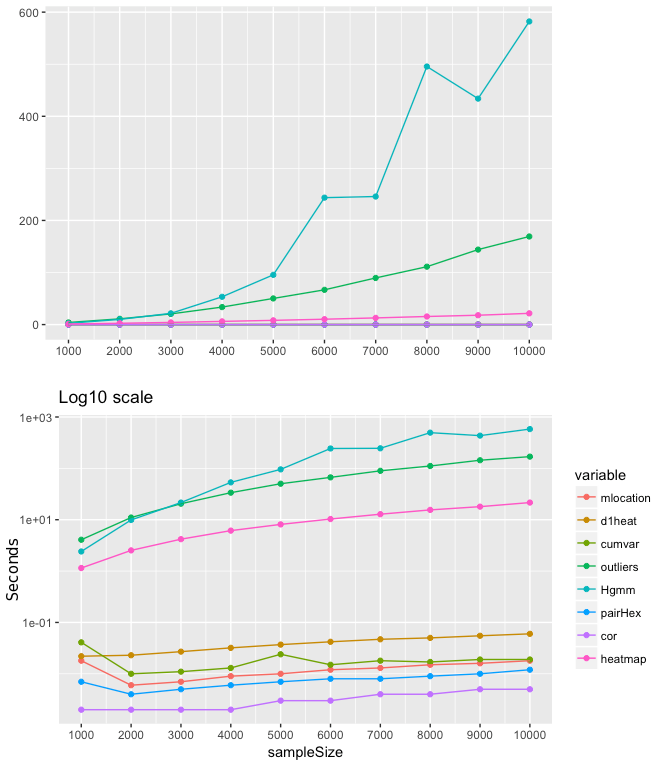
\includegraphics[width=0.6\textwidth]{../../figs/medaTimeTest.png}
%\caption{Timing plots for the functions used in meda.  The bottom plot
%  is the log scale of the top one. The data used consisted of 10,000
%  observations in 24 dimensions, sampled in chunks of inceasing size.
%  The Hgmm function takes about 10 minutes  on the largest sample used.}
%\label{fig:medaTimeTest}
%\end{cframed}
%\end{figure}
%
%\clearpage

%% May

A docker container
\href{https://hub.docker.com/r/neurodata/synaptograms/}{https://hub.docker.com/r/neurodata/synaptograms/}
has been developed to view multi-channel
muti-dimensional image data.  Array tomography (AT) provides a good
use-case. AT data consist of (3+$c$)-dimensional data, where $c$ is the
number of features/channels collected. 
%
A putative synapse location corresponds to an 11x11x11
pixel cube in the image and this cube will have multiple corresponding
channels. These channels can express the presence or absence of a
certain protein marker such as Synapsin or VGlut2. 

\begin{figure}[!h]
\begin{cframed}
\centering
\includegraphics[width=0.98\textwidth, clip = true, trim = 0in 18in 0in 0in]{../../figs/exampleC1212testkristina15x108_y5965_z22.png}
\caption{
  Using a synapse detection algorithm we believe that there is a synapse
  at this location.  The location is defined by an 11x11x11 cube with 11
  feature channels. Each row of the figure corresponds to the cube over
  a specific feature channel.  The cube has been splayed out in the
  z-direction over the columns. The far right column corresponds to the
  sum statistic of each row.  This plot enables viewing of an
  11x11x11x$c$ object nicely on screen, where $c$ in this case happens
  to be 11. 
}
\label{fig:meda:synaptogram}
\end{cframed}
\end{figure}


\end{document}
